\textbf{X -- ALTRI ASPETTI}

\textbf{DELLA BATTAGLIA SCACCHISTICA}

\textbf{a) L'aspetto psicologico}

``Io gioco contro la posizione, non contro l'avversario'' si sente dire
sovente in quella che è più una dichiarazione d'intenti che una realtà.
Se questo atteggiamento di fronte alla scacchiera è una ricerca di
obiettività allora siamo d'acco¢do ma se invece si intende che non si
rimane influenzati da chi si ha di fronte e da tutto il contorno, ho
l'impressione che sia una pia illusione e, in una certa misura, anche
una falsità.

Chi infatti si asterrebbe da giocare una novità teorica, a lungo
preparata in analisi casalinghe, per giocare la variante considerata
migliore dalla teoria e che sappiamo essere ben conosciuta
dall'avversario?

Nella dodicesima partita del campionato del mondo del 1985, Garry
Kasparov non esitò a giocare l'interessante ma dubbio gambetto che
avrebbe poi preso il suo nome. Fu una mossa calibrata su misura per
Karpov, dove più che la ``verità'' scacchistica contava il vantaggio di
giocare una variante ben studiata e soprattutto inedita. Karpov riuscì a
pattare quella partita e forse non si aspettava che lo sfidante
riproponesse il sacrificio, come invece accadde, nella sedicesima. Il
colpo riuscì e Kasparov vinse una importante partita, vera svolta
psicologica della sfida.

Il primo a teorizzare l'arma psicologica negli scacchi fu Emanuel
Lasker, campione del mondo dal 1894 al 1921. Egli giocò esplicitamente
tenendo conto delle caratteristiche psicologiche dell'avversario e
grazie ad esse colse innumerevoli successi. Buona parte delle sue
partite erano perse poco dopo l'apertura ma, tra la sorpresa generale,
riusciva a vincerle.

Gli errori psicologici che si possono commettere sono molti. Quello di
partire sconfitti è un atteggiamento più comune di quel che si immagini
e porta a fare mosse rinunciatarie o giocare mosse rischiose senza un
calcolo adeguato: ``Tanto perdo lo stesso'', si pensa in questi casi.
Bisogna imparare a affrontare i giocatori più forti col massimo impegno;
le partite con essi devono essere di stimolo, non di sconforto.

Un altro atteggiamento sbagliato, di cui sono stato vittima anch'io, è
farsi cogliere dal panico in caso di una mossa inaspettata. Ho imparato
tardi come fare; un tempo ero solito rispondere subito a una mossa
imprevista per non mostrare di essere stato colto di sorpresa, e così,
spesso e volentieri, pe¢devo non tanto per la forza della mossa
imprevista quanto piuttosto dell'errore nella risposta non ponderata.

Questo modo di fare era così spontaneo che non mi rendevo nemmeno conto
di averlo. Scoperto il difetto mi imposi, dopo una mossa imprevista, di
guardare il soffitto e contare fino a dieci prima di immergermi nelle
analisi. Questo inusuale atteggiamento doveva apparire buffo ai miei
avversari ma la cosa funzionò e imparai ben presto a correggere il
difetto.

Le mosse inaspettate, quando buone, non sono incidenti di percorso come
credono molti scacchisti ma devono suonare come un campanello di
allarme. Possono semplicemente essere sintomo di stanchezza ed allora,
mentre l'avversario pensa, è bene alzarsi e fare un giro nella sala di
gioco per distrarsi un po', ma possono anche essere rivelatrici di
lacune tattiche o strategiche.

Per questo la posizione precedente alla mossa che ci ha sorpreso va
sempre riesaminata con cura cercando di capire i motivi che hanno reso
ciechi.

Talvolta si diventa ``ciechi'' in seguito a una costante iniziativa. Si
desidera così tanto trovare la continuazione vincente che si finisce col
pensare solo a mosse d'attacco e si trascurano le minacce avversarie. In
questi casi, se i danni non sono irreparabili, la mossa imprevista può
avere l'effetto salutare di un ritorno alla realtà.

Ma, in generale, non è bene scherzare col fuoco, occorre imparare a
mantenersi sempre distaccati e obiettivi di fronte a qualsiasi
posizione. Ecco, se una cosa insegnano gli scacchi questa è
l'obiettività: gli scacchi sono una delle poche attività umane dove non
si fanno progressi se non si impara ad essere obiettivi e moderati nei
giudizi. Da questo punto di vista sono veramente una palestra in cui si
verificano continuamente le idee proprie e altrui. Chi fa affermazioni a
priori, chi si incaponisce nel dimostrare l'indimostrabile va incontro a
cocenti sconfitte.

Il grande maestro tedesco Uhlmann continuò per un pezzo a giocare una
certa variante della Francese incurante che fossero state trovare linee
molto buone per il Bianco e naturalmente pe¢deva una partita dietro
l'altra. A chi gli chiedeva come mai continuasse a giocare una linea
palesemente sbagliata rispondeva: ``Perché non ho fatto altro per tutta
la vita!''

Anch'io una volta, per una semplice questione di ripicca, mi esposi al
rischio di una variante preparata. Il mio avversario sapeva che cosa
avrei giocato e, solo per un malinteso senso dell'orgoglio, per
dimostrare che una vittoria conseguita in precedenza proprio contro di
lui non era stata frutto del caso, decisi che non mi sarei tirato
indietro.

Quella volta andò bene ma non è consigliabile riprovarci.

Vediamo quel che successe in quelle due partite.

Gongalov--Leoncini, Imperia 1987 \textbf{(Difesa Siciliana)}

\textbf{1.e4 c5 2.¤f3 ¤c6 3.d4 ¤xd4 4.¤xd4 ¤f6 5. ¤c3 e5 6.C£d5} la
migliore continuazione. Altre mosse di Cavallo sono meno incisive: 6.¤f5
d5!; 6.¤f3 ¥b4; 6. \textbf{¤}de2 ¥b4.

\textbf{6... .d6 7.¥g5} con 7.¤d5 ¤xd5 8.exd5 ¤b8 9.c4 il Bianco
rinuncia allo sfruttamento del buco in d5 e del pedone debole in d6 per
valorizzare la maggioranza di pedoni ad ovest.

\textbf{7... .a6 8.¤a3 b5 9.¥xf6} il Bianco può mantenere la partita su
binari posizionali giocando 9.¤d5 ¥e7 10..¥xf6. La scelta di una
variante dipende in larga misura dall'indole del giocatore.

\textbf{9... gxf6 10.¤d5 f5 11.¥xb5} è interessante anche l'altro
sacrificio di pezzo in b5: 11.¤xb5 axb5 12.¥xb5 ¥b7 13.exf5 ma
l'esperienza mi ha portato a temere di più continuazioni solide come
11.¥d3 o 11.exf5. Gongalov eseguì il sacrificio con l'aria come per dire
``Ora ti sistemo io!''.

\textbf{11... axb5 12.¤xb5 £g5} la teoria considera migliore 12... ¦a4
ma anche la continuazione del testo conduce a posizioni taglienti e ha
il vantaggio di essere meno studiata.

\emph{diagramma 112}

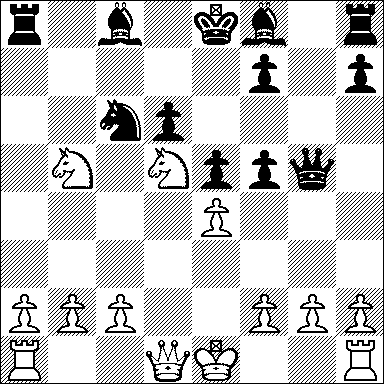
\includegraphics[width=1.40139in,height=1.40139in]{assets/diagrams/image112.png}

\textbf{13.¤bc7+} il Cavallo sbagliato. Questa mossa è buona su 12...
¦a4 mentre qui non è granché. Sempre su 12... ¦a4 è invece sbagliata 13.
\textbf{¤}dc7+ che qui è buona. Insomma, la scelta di una variante
minore (12... £g5) ha dato i suoi frutti. Per 12. \textbf{¤}dc7 si veda
la partita successiva.

\textbf{13... ¢d8 14.¤xa8 £xg2 15.¦f1 £xe4+ 16.¤e3 ¤d4 a}ll'immediata
16... f4? sarebbe seguito 17.£d5.

\textbf{17.¤b6 f4 18.c3 ¤f3+ 19.¢e2 fxe3 20.fxe3 ¤d4+} minaccia 21...
¥g4+.

\textbf{21.¢d2 ¥g4} la posizione del Bianco è insostenibile.

\textbf{22.£xg4} non c'è altro. 22.£a4 £g2+ 23.¢d3 ¥e2+ 24.¢d2 ¥b5+.

\textbf{22\ldots£xg4 23.¤xd4 exd4 24.¦ac1 £xe3+ 25.¢d3 £g6+} non c'è più
storia.

\textbf{26.¢d4 ¥g7+ 27.¢d5 £e6+ 28.¢c6 ¦e8 29.¤d5 £d7+ 30.¢b6 ¥d4+
31.¢a5 ¦e5 32.} il Bianco abbandona.

Alla fine della partita Gongalov era irritato per aver perso contro una
variante a suo avviso insostenibile. Il caso volle che due anni dopo ci
si trovasse di fronte con gli stessi colori.

Gongalov--Leoncini, Imperia 1989 \textbf{(Difesa Siciliana)}

Le prime dodici mosse come nella partita precedente.

\textbf{13. ¤dc7+} stavolta il Bianco si preparato a dovere e dà lo
scacco in c7 col Cavallo giusto.

\textbf{13... ¢d8} questa partita venne giocata all'ultimo turno ed era
di rilievo per la classifica. Seppi poi che a questo punto molti mi
davano per spacciato. Io, invece, anche se feci una lunga riflessione
per richiamare le cognizioni teoriche sapevo bene che la partita era
ancora tutta da giocare.

\textbf{14.£d5 ¥b7 15.£xf7} è migliore 15.¤xa8 ¥xa8 16.£xf7 ¥e7 17.£xf3
£xf5 18.exf5. In una mia partita precedente seguì 18... ¦g8 19.0-0-0 ¤d4
20.¤xd4 exd4 21.¦xd4 ¦xg2 22.¦hd1 ¦xf2 23.¦xd6+ ¥xd6 24.¦xd6+ ¢e8 25.¦h6
¥e4 26.¦xh7 ¦xc2+ 27.¢d1 ¥xf5 patta (Lucaroni--Loncini, Gaeta 1986).

\textbf{15... £e7 16.£d5} con 16.¤xa8 ¥xa8 17.£xf7 si rientrava nella
variante di cui alla nota precedente. Dopo la mossa del teso il Nero
salva la Torre.

\textbf{16... ¦c8 17.¤e6+ ¢e8 18.0-0-0 ¤d4 19.¤xd6+ £xd6 20.¤g7+ ¢d8
21.£a5+?} è meglio 21.¤e6+ sperando nella divisione del punto anche se
il Nero potrebbe tentare 22... ¢e8 23.¤g7+ ¢e7 24.£xb7+ ¦c7 25.¤xf5 ¤xf5
26.¦xd6 ¦xc7.

\textbf{21... ¦c7} non 21... £c7?? per 22.¤e6+ e cala il sipario.

\textbf{22.¤xf5 £c5 23.¤xd4 exd4} se 23... £xa5 24.¤c6+ e poi 25.¤xa5.

\textbf{24.£d2 ¥h6!}

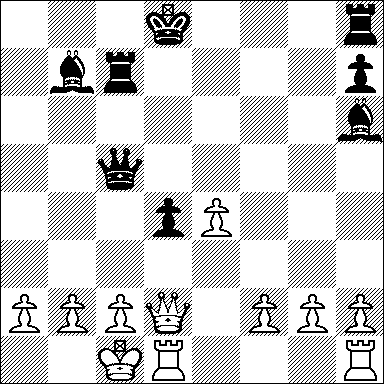
\includegraphics[width=1.40139in,height=1.40139in]{assets/diagrams/image113.png}

\emph{diagramma 113}

La mazzata finale: se 25.£xh6 £xc2 matto.

\textbf{25. il Bianco abbandona.}

Chiudo qui queste brevi note ma chi fosse interessato ad avere un
atteggiamento \emph{sano} durante un torneo, può leggere la tesi di
laurea in psicologia del grande maestro N. V. Krogius, tradotta in
italiano da Roberto Paniagua, e pubblicata con il titolo ``Scacchi e
creatività'' (Abano Terme, Francisci editiore, pp. 109, 1984) oppure il
lavoro di Hartston e Wason ``¦he Psychology of chess'' (London,
Batsfo¢d, pp. 138, 1983).

\textbf{b) Gli scacchi come lotta}

Gli scacchi competitivi non sono un balocco, un gioco con cui ci si
trastulla e si passano ore piacevoli e spensierate. Sono una
competizione intellettuale dura anche se costellata di bellezza. Questo
potrà scandalizzare molti puristi del gioco e certi moralisti.

Komeini li proibì e anche il famoso educatore don Lorenzo Milani
redarguì con severità due allievi trovati intenti a giocare a scacchi e
così si espresse sull'argomento in una famosa lettera: \emph{``E non si
gioca a scacchi mai, perché non esiste gioco più profondamente immorale
laddoveché richiede concentrazione intellettuale, mentre un gioco, anche
a volerlo concedere, ma non lo concederei neanche così, deve essere
almeno distensivo''} (Lettera a V. Lampronti).

A queste opinioni ne fanno da contrappunto altre più rassicuranti:
``Come l'amore e come la musica, gli scacchi hanno il potere di far
felici gli uomini'' ebbe a dire Siegberg Tarrasch; oppure:
\emph{``Andando sulla Luna l'uomo si è avvicinato agli dei, giocando a
scacchi egli è da tanto tempo con loro''.}

La bellezza negli scacchi, per quanto scaturisca da aspetti razionali e
misurabili, li accomuna all'arte ma la competizione spinta li fa
assomigliare a uno sport.

Nei tornei di un certo livello questi due aspetti sono entrambi
presenti. Quello che tanto attrae in questo gioco a informazione
completa, e dove la fortuna ha un ruolo marginale, è mettere le proprie
capacità a confronto con quelle di altri. In questo senso la vittoria
equivale a un'iniezione di fiducia in se stessi purché non costellata da
errori propri o grossolanità dell'avversario. Altrimenti rimane sempre
un quid di insoddisfazione.

Alekhine si lamentava degli errori degli avversari che non gli
consentivano di creare quei capolavori della scacchiera che desiderava e
intravedeva; e chi, partecipando a un torneo, non ha mai visto un
giocatore scuotere il capo e dire sconsolato: ``Ho vinto ma ho giocato
male''.

Il maestro genovese Federico Cirabisi è noto per giocare con spirito
Romantico. Alla fine di un torneo disastroso egli può essere il
giocatore più felice del torneo purché sia riuscito a giocare una
partita da ``premio di bellezza''.

Nella partita che segue i giocatori si affrontano a viso aperto in una
lotta avvincente.

Kortchnoi--Kasparov, Olimpiadi di Lucerna 1982 \textbf{(Difesa Benoni)}

\textbf{1.d4 ¤f6 2.c4 g6} Kasparov scrive: \emph{``Conscio del fatto che
l'esperienza di Kortchnoi in molti sistemi di apertura è
incomparabilmente più vasta della mia, scelsi l'Est Indiana, una difesa
che ho sempre studiato a fondo''}.

\textbf{3.g3 ¥g7 4.¥g2 c5} Kasparov: \emph{``Il fianchetto dell'Alfiere
campochiaro da parte del Bianco è molto spiacevole per il Nero nelle
linee classiche dell'Est Indiana, ma meno incisivo contro alcune
varianti della Benoni. Ciò spiega la scelta del Nero''.}

\textbf{5.d5 d6 6.¤c3 0-0 7.¤f3 e6 8.0-0 exd5 9.¤xd5 a6 10.a4 ¦e8 11.¤d2
¤bd7 12.h3 ¦b8 13.¤c4 ¤e5} meno ambiziosa, ma forse più in linea con lo
spirito della variante, è 13... ¤b6 ma Kasparov intende giocare a tutto
campo.

\textbf{14.¤a3 ch5 15.e4} in caso di 15.f4 il Nero avrebbe sacrificato
il Cavallo in g3 16.fxe5 ¥xe5. Dopo 15.g4 avrebbe invece lasciato al suo
destino il ch5 e giocato 15... £h4 16.hxg5 ¥xh3.

\textbf{15... ¦f8 16.¢h2 f5 17.f4}

\emph{diagramma 114}

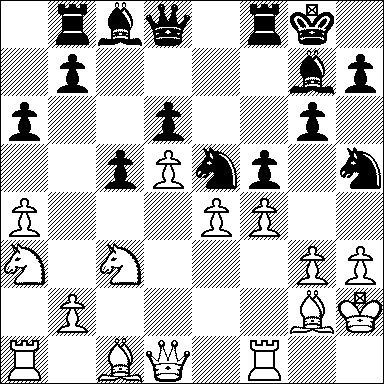
\includegraphics[width=1.40139in,height=1.40139in]{assets/diagrams/image114.png}

\textbf{17... b5} bellissima: tutta la scacchiera entra il
fibrillazione.

\textbf{18.axb5} la cattura del Cavallo avrebbe condotto a complicazioni
tremende ma probabilmente favorevoli al Nero dopo 18.fxe5 ¤xg3!
\emph{(meglio di 18... ¥xe5 19.¤e2!)} 19.¢xg3 ¥xe5+ 20.¢f3 \emph{(20.¢f2
£h4+ 21.¢g1 ¥xh3 22.£e1 ¥g3 23.¦f4 ¥g4)} 20... b4.

\textbf{18... axb5 19.¤axb5 fxe4 20.¥xe4} il Cavallo è ancora
intoccabile: 20.fxe5 ¥xe5 21.¥f4 ¤xf4 22.gxf4 ¥xf4+ 23.¢g1 ¥d7.

\textbf{20... ¥d7!} Splendido! Oltre al Cavallo Kasparov lascia in presa
anche il Pd6!

\textbf{21.£e2} su 21.¤xd6 il Nero aveva preparato 21... ¦b6! 22.fxe5
¥xe5 23.¤c4 ¥xg3+ 24.¢g1 ¦bf6 25.¥g2 ¦f2 con attacco fortissimo.

\textbf{21... £d6 22.¤a3 ¦be8 23.¥d2 £xb2 24.fex5?} non reggendo la
tensione. Si doveva giocare 24.¦a2, ora il Nero dilaga.

\textbf{24... ¥xe5 25.¤c4 ¤xg3! 26.¦xf8+ ¦xf8 27.£e1 ¤xe4+ 28.¢g2 £c2}
Kasparov poteva chiudere subito con 28... ¦f2+! 29,£xf2 (29.¦h1 ¦xd2!)
29... ¥xh3+ 30.¢f3 ¤xd2 31.£xd2 £xa1 32.¤xe5 £xe5.

\textbf{29.¤xe5 ¦f2?} le terribili complicazioni fanno pe¢dere la
bussola anche al futuro campione del mondo. Si vinceva con 29... ¤xd2!
30.¤xd7 ¤f3 31.£e2 ch4+ 32.¢g1 £xc3 33.£e6+ ¢h8 34.¤xf8 £g3+ 35.¢f1 £g2+
36.¢e1 ¤f3+ 37.¢d1 £d2~matto. Incalzato dal tempo al Nero sfugge la
forza del prossimo sacrificio di Donna di Kortchnoi.

\textbf{30.£xf2! ¤xf2 31.¦a2 £f5 32.¤xd7 ¤d3 33.¥h6?} una maggiore
resistenza avrebbe offerto 33.¦a8+ ¢g7 34.¦a7 con complicazioni.

\textbf{33... £xd7 34.¦a8+ ¢f7 35.¦h8 ¢f6 36.¢f3??} un erroraccio in
zeitnot in posizione perduta.

\textbf{36... £xh3+ 37. il Bianco abbandona.}

\emph{``Gli scacchi sono uno sport''} ebbe a dire una volta il noto
pittore francese Marcel Duchamp \emph{``uno sport violento''.} E pur nel
paradosso forse colse un'importante verità.

Ci sono giocatori che fanno di ogni partita un'avventura epica, Kasparov
e Kortchnoi rientrano in questa categoria e non a caso i loro incontri
sono particolarmente combattuti; altri, come lo fu in sommo grado
Capablanca, che invece sembrano ridurre tutto a una questione di
migliore strategia.

Indipendentemente dall'indole del giocatore (semmai egli si costruirà un
repertorio che rispecchi il suo modo di vedere gli scacchi) talune
aperture conducono a partite di grande complessità. È il caso di £g4
nella Variante Vinawer della difesa Francese, e la partita che segue ne
è un esempio.

Entrambi i giocatori sono alla ricerca costante dell'iniziativa ed è
difficile dire, in qualsiasi momento, chi tenga le redini della partita.
Solo all'entrata in finale le cose si chiariscono e il Bianco in pochi
tratti efficaci evita al Nero una lunga agonia.

Leoncini--Mazzotti, Imperia 1989 \textbf{(Difesa Francese)}

\textbf{1.e4 e6 2.d4 d5 3.¤c3} un'alternativa, di certo più posizionale,
è 3.¤d2.

\textbf{3... ¥b4} una mossa introdotta da Nimzowitsch. L'alternativa più
comune è 3... ¤f6.

\textbf{4.e5 c5 5.a3 ¥xc3+ 6.bxc3 ¤e7} la variante Winawer, una delle
più movimentate della Francese.

\textbf{7.£g4} il Bianco sarebbe stato ancora in tempo a giocare in
stile più posizionale con 7.¤f3. È degna di interesse la mossa riesumata
da Short 7.h4, con l'idea di spingere il pedone fino a h6 e indebolire
ulteriormente le case nere, visto che il Nero si è privato dell'Alfiere
campo scuro.

\textbf{7... £c7} la teoria considera 7... 0-0 8.¤f3 ¤c6 9.¥d3 f5
10.exf6 ¦xf6 11.¥g5 ¦f7 leggermente favorevole al Bianco. In caso di
11... e5 la seconda edizione del Batsford chess Openings consiglia
12.¥xh7+ ¢xh7 13.£h5+ ¢g8 14.¥xf6 gxf6 l5.£xe5 con vantaggio del Bianco
ma dopo 15... £f8 16.0-0 £f7 17.£xf7+ ¢xf7 18.¦fel ¥f5 il vantaggio, sia
pure lieve, sembra piuttosto dalla parte del Nero. Probabilmente, dopo
11... e5, il Bianco deve giocare 12.£h4 e4 13.¥xf6 gxf6 14.£xf6 exd3
15.¤xd3 ¥f5 16.0-0! ¥xd3 17.£e6+ ¢g7 18.¤e5 con una certa iniziativa
(18... ¥xf1?? 19.£f7+ ¢h8 {[}19..¢h6 20.£f6+!{]} 20.£f6+ ¢g8 21.¤f7 £f8
22. \textbf{¤}h6+).

\textbf{8.£xg7 ¦g8 9.£xh7 ¤xd4 10.¤e2 ¤bc6 11.f4 ¥d7 12.£d3 £xc3
13.¤xc3} il Bianco ha un pedone in più ma il suo Re è rimasto al centro.

\textbf{13... a6 14.¤e2 ¤a5 15.¤d4 0-0-0 16.¦b1 ¤ec6 17.¤xc6 ¥xc6
18.£d4} occorre evitare la spinta in d4 che aprirebbe la grande
diagonale all'¥c6.

\textbf{18... ¤c4 19.¢f2 £e7} il Nero si prepara ad aprire il centro.
L'apertura del centro è la corretta strategia quando l'avversario si è
privato dell'arrocco.

\textbf{20.¦b3} il teatro delle operazioni si sta spostando sul lato di
Re e questa Torre accorre a dar man forte alla fortificazione bianca.

\textbf{20... ¦g6 21.¦f3 ¦dg8 22.g3 f6} piazzati i pezzi in posizione di
attacco il Nero rompe gli indugi ma la cittadella bianca sembra ben
difesa.

\textbf{23.h3 £g7 24.exf6 ¦xf6 25.¦g1 e5} ancora una spinta di rottura.

\textbf{26.£a7} il Bianco mantiene il controllo dell'importante
diagonale a7-g1 e inoltre, in caso di 26... exf4 27.¥xf4, è pronto a
penetrare nelle retrovie nemiche con £d8+.

\textbf{26... e4 27.¦c3!} inchioda in modo preventivo l'¥c6.

\textbf{27... e3+ 28.¥xe3 ¤xe3 29.£xe3 ¦xf4+ 30.gxf4} più semplice di
30.£xf4 ¦f8.

\textbf{30... £xg1 31.¢e1 d4 32.£xg1 ¦xg1 33.¦c5 ¦g3 34.¥xa6}
l'importanza della Torre sulla colonna c!

\textbf{34... bxa6 35.¦xc6+ ¢b7 36.¦d6 ¦xh3 37.¦xd4 ¦xa3} la situazione
si è chiarita: il Bianco è rimasto col pedone in più e nutre grosse
speranze di vittoria grazie ai due pedoni liberi e distanti dall'unico
pedone nero.

\emph{diagramma 115}

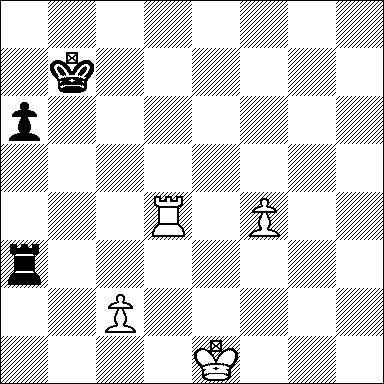
\includegraphics[width=1.40139in,height=1.40139in]{assets/diagrams/image115.png}

\textbf{38.¦d3!} com'è noto, in questo tipo di finali, la posizione
corretta della Torre è dietro al pedone che deve essere spinto.

\textbf{38... ¦a4 39.¦f3 ¦e4+ 40.¢d2 ¢c6 41.f5} la mossa in busta e
l'inizio del piano giusto.

\textbf{41... ¦e8 42.f6 ¦f8 43.f7} con la Torre nera praticamente fuori
gioco, vincere diventa facile.

\textbf{43... ¢d5 44.¢c3} il Bianco si appresta a catturare l'ultimo
pedone nero.

\textbf{44... a5 45.¢b3 ¢e4 46.¦f6 ¢d4 47.¢a4 ¢c5 48.¦f5+} 48.¢xa5 ¦a8
matto e quella notte non avrei dormito!

\textbf{48... ¢b6 49.c3} Zugzwang. I pezzi neri sono già piazzati nelle
loro case migliori ma qualcosa deve pur essere mosso.

\textbf{49... ¢c6 50.¢xa5 ¦a8+ 51.¢b4 ¦b8+ 52.¢c4 ¦f8 53.¢d4 ¢d6 54.¦f6+
¢e7 55.¢e5 ¢d7 56.¦f4 ¢e7 57.c4} di nuovo una posizione di zugzwang.
L'entrata del Re bianco in f6 decide la partita.

\textbf{57... ¢d7 58.¢f6 il Nero abbandona.}

Abbiamo accennato alla bellezza degli scacchi. I criteri per definirla
non sono facili ma come non considerare bella la partita giocata dal
grande Alekhine, col suo stile volitivo, contro il connazionale Efim
Bogoljubov?

Bogoljubov--Alekhine, Hastings 1922 \textbf{(Difesa Olandese)}

\textbf{1.d4 f5} per evitare il fastidioso Gambetto Staunton (2.e4)
alcuni preferiscono far precedere questa mossa da 1... e6 ma devono
essere pronti a giocare la Francese in caso di 2.e4.

\textbf{2.c4 ¤f6 3.g3} l'Alfiere di Re nell'Olandese trova adeguata
sistemazione in fianchetto; quello nero, invece ha problemi di sviluppo.
Se il Nero adotta lo Stonewall (c6-d5-e6-f5) può trovare sfogo nella
diagonale d1-h5 con la manovra d7-e8-h5. In questa partita Alekhine
decide, invece, di arrivare al più presto alla spinta in e5.

\textbf{3... e6 4.¥g2 ¥b4+} se il Bianco desidera evitare le varianti
che si dipanano da questo scacco può ritardare la spinta in c4 a dopo
l'arrocco (2.g3 e6 3.¥g2 ¤f6 4.¤f3 ¥e7 5.0-0 0-0 6.c4).

\textbf{5.¥d2 ¥xd2+ 6.¤xd2 ¤c6 7.¤gf3 0-0 8.0-0 d6 9.£d3 ¢h8 10.£c3}
spostandosi sulla diagonale del Re, la Donna sembra fare la corte al Re
nemico. Il Nero minaccia l'espansione ad ovest con b4 e forse, guardando
col terzo pezzo in e5, si intendeva evitare tale spinta.

\textbf{10... e5!} Alekhine effettua lo stesso la spinta in
considerazione che il ¤d2, dopo le ripetute prese in e5 rimane indifeso.

\textbf{11.e3 a5} per ritardare l'espansione bianca sul lato di Donna.

\textbf{12.b3 £e8} l'¥g2 e la struttura dei pedoni bianca impongono
un'iniziativa del Bianco sul lato di Donna mentre la catena di pedoni
(c7-d6-e5-f5) indicano al Nero di attaccare sul lato di Re.

\textbf{13.a3 £h5!} il Pe5 è ancora intoccabile. Dopo 14.£xe5 £xe5
15.¤xe5 ¤xe5 16.£xe5?? il Nero vince di colpo con 16... ¤g4, con il
doppio attacco alla Donna e al matto in h2.

\textbf{14.h4 ¤g4 15.¤g5 ¥d7 16.f3} il Pe5 è ancora imprendibile. Dopo
16.¥xc6 ¥xc6 17.f3 exd4 18.fxg4 £xc3 19.gxh5 ¤xd2 il Nero è in
vantaggio.

\textbf{16... ¤f6 17.f4} la minaccia di spingere in f4 costringe il
Bianco a un ulteriore indebolimento.

\textbf{17... e4 18.¦fd1 h6 19.ch3 d5 20.¤f1 ¤e7 21.a4 ¤c6 22.¦d2 ¤b4
23.¥h1 £e8!} all'iniziativa nera sul lato di Re il Bianco non è riuscito
a contrapporne una altrettanto efficace sul lato opposto. Alekhine,
maestro nel giocare a tutto campo, cambia all'improvviso fronte e va a
sfruttare le debolezze bianche sul lato di Donna.

\textbf{24.¦g2 £xc4 25.bxc4 ¥xa4 26.¤f2 ¥d7 27.¤d2 b5! 28.¤d1 ¤d3
29.¦xa5}

\emph{diagramma 116}

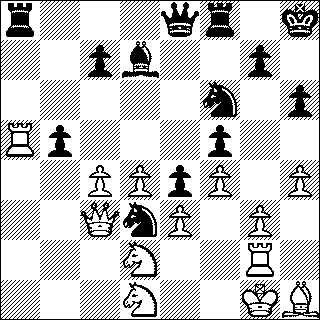
\includegraphics[width=1.33889in,height=1.33889in]{assets/diagrams/image116.png}

\textbf{29... b4! 30.¦xa8} Pachman propone 30.£a1 ma Kotov fa notare che
dopo 30... ¦xa5 31.£xa5 £a8! 32.£xa8 ¦xa8 l'irruzione della Torre nera
decide rapidamente.

\textbf{30... bxc3 31.¦xe8 c2!} una mossa che è un monumento al pedone
libero. Non c'è modo di impedire la promozione. In genere le due Torri
valgono più della Donna ma in questo caso la mancanza di coordinazione
fa pendere la bilancia dalla parte del Nero.

\textbf{32.¦xf8+ ¢h7 33.¤f2 c1=£+ 34.¤f1 ¤e1 35.¦h2 £xc4 36.¦b8 ¥b5
37.¦xb5} non c'è altro. Ora il Nero è anche in vantaggio di materiale.

\textbf{37... £xb5 38.g4 ¤f3+ 39.¥xf3 exf3 40.gxf5 £e2!} una bellissima
posizione di zugzwang! Il Bianco non può muovere alcun pezzo senza
perdere materiale, rimangono le mosse di pedone e Alekhine aspetterà
semplicemente che si esauriscano!

\textbf{41.d5} 41.ch3 non va per 41... ¤g4.

\textbf{41... ¢g8 42.hS ¢h7 43.e4 ¤xe4 44.¤xe4 £xe4 45.d6 ¤xd6 46.f6
gxf6 47.¦d2 £e2} questo nuovo sacrificio di Donna serve a forzare
l'entrata in un finale di pedoni facilmente vinto.

48.¦xe2 fxe2 49.¢f2 exf1=\textbf{£}+ 50.¢xfl ¢g7 51.¢e2 ¢f7 52.¢e3 ¢e6
53.¢e4 d5+ 54. il Bianco abbandona.

\textbf{c) Come prepararsi a un torneo di scacchi}

Ci sono giocatori che disputano un torneo dietro l'altro senza alcuna
preparazione, come andassero in villeggiatura. Eppure, più che giocare
tantissimo è importante giocare con la massima serietà i tornei cui si
decide di partecipare.

Se si desiderano ottenere risultati occorre un minimo di preparazione,
dove per minimo si deve intendere:

1) controllare le linee di apertura che si è soliti giocare, sia per
rinfrescare la memoria che per valutare eventuali novità teoriche
introdotte nella pratica dei tornei;

2) analizzare le proprie partite dei tornei precedenti, in modo speciale
quelle perdute. Trovare gli errori e formulare il piano corretto;

3) se possibile, ma non strettamente necessario, giocare una o due
partite di allenamento con un giocatore di forza pari o maggiore, col
tempo previsto dal bando di gara del torneo cui si intende partecipare.

Nella trasferta non occorre portarsi dietro l'intera Enciclopedia degli
Scacchi, basta un buon libro di teoria delle aperture; inoltre è bene
avere un con sé un libro sui finali, nel caso che la partita venga
sospesa.

Quando si partecipa ad un torneo di forza magistrale è utile disporre di
un computer portatile con un \emph{database} elettronico per conoscere
in anticipo le aperture degli avversari. In mancanza di un computer si
può facilmente creare un proprio schedario annotando le aperture che
giocano gli altri partecipanti ai tornei ai quali si partecipa; il data
base può servire anche come ausilio per lo studio.

A costi non eccessivi il mercato ne offre diversi, tutti ormai piuttosto
sofisticati e con centinaia di migliaia di partite già disponibili.

Le funzioni principale di un data base di scacchi sono:

a) ricerca delle partite per giocatore, per torneo, per anno, per
vittoria del Bianco o del Nero, per numero di mosse, per punteggio Elo
ecc., anche mischiando i vari criteri;

b) per variante d'apertura;

c) per ``motivo'' (per es.: sacrificio di Cavallo in b5);

d) per tipo di finale (per es.: Torre e pedone contro Torre e due
pedoni).

Durante il torneo:

a) imparare a non muovere mai senza aver riflettuto, anche se la mossa è
evidente o addirittura forzata;

b) amministrare il proprio tempo per evitare di rimanerne a corto;

c) non prendersela in caso di sconfitta; ricordarsi che ogni partita fa
storia a sé.

\clearpage
\onecolumn
INDICE

\begin{longtable}[]{@{}
  >{\raggedright\arraybackslash}p{(\columnwidth - 2\tabcolsep) * \real{0.50}}
  >{\raggedright\arraybackslash}p{(\columnwidth - 2\tabcolsep) * \real{0.50}}@{}}
\toprule
\endhead
Introduzione & 3 \\
I -- Sviluppo dei pezzi e perdita di tempi & 6 \\
\begin{minipage}[t]{\linewidth}\raggedright
II -- Un metodo per avvantaggiarsi in apertura: il gambetto

\begin{enumerate}
\def\labelenumi{\arabic{enumi}.}
\item
  Sacrifici operati dal Bianco
\item
  Sacrifici operati dal Nero
\end{enumerate}
\end{minipage} & 15

17

21 \\
\begin{minipage}[t]{\linewidth}\raggedright
III -- La struttura dei pedoni

\begin{enumerate}
\def\labelenumi{\arabic{enumi}.}
\item
  l'indebolimento delle case e il ``buco'' (``foro'', ``hole'')
\item
  I pedoni deboli

  \begin{enumerate}
  \def\labelenumii{\alph{enumii}.}
  \item
    Il pedone isolato
  \item
    Il pedone arretrato
  \item
    Pedoni doppiati (o impedonati)
  \item
    Pedoni sospesi
  \end{enumerate}
\end{enumerate}

\begin{enumerate}
\def\labelenumi{\arabic{enumi}.}
\setcounter{enumi}{2}
\item
  L'attacco di minoranza

  \begin{enumerate}
  \def\labelenumii{\alph{enumii}.}
  \item
    Contrattacco a un attacco di minoranza
  \item
    Contrastare `attacco sullo stesso lato
  \end{enumerate}
\item
  I pedoni forti

  \begin{enumerate}
  \def\labelenumii{\alph{enumii}.}
  \item
    Il pedone passato isolato
  \item
    Il pedone passato sostenuto
  \end{enumerate}
\end{enumerate}

5. L'attacco di maggioranza

Appendice al capitolo III
\end{minipage} & 30

30

36

36

39

44

50

53

56

59

64

65

66

72

77 \\
\begin{minipage}[t]{\linewidth}\raggedright
IV -- Gli avamposti

\begin{enumerate}
\def\labelenumi{\alph{enumi})}
\item
  Il caso del pedone
\item
  Il caso del pezzo
\end{enumerate}
\end{minipage} & 82

82

83 \\
\begin{minipage}[t]{\linewidth}\raggedright
V -- Attacco e contrattacco

\begin{enumerate}
\def\labelenumi{\arabic{enumi}.}
\item
  Gli attacchi eterogenei
\item
  L'indebolimento dell'arrocco

  \begin{enumerate}
  \def\labelenumii{\alph{enumii}.}
  \item
    indebolimento per spinta di pedoni
  \item
    Indebolimento per rimozione di pezzi
  \item
    Il Re al centro
  \end{enumerate}
\end{enumerate}
\end{minipage} & 88

92

97

97

101

103 \\
\begin{minipage}[t]{\linewidth}\raggedright
VI -- La colonna aperta

\begin{enumerate}
\def\labelenumi{\alph{enumi}.}
\item
  La settima traversa
\item
  Debolezza dell'ottava traversa
\item
  Il punto d'appoggio
\end{enumerate}
\end{minipage} & 108

108

112

115 \\
\begin{minipage}[t]{\linewidth}\raggedright
VII -- Gli Alfieri

\begin{enumerate}
\def\labelenumi{\alph{enumi})}
\item
  La coppia degli Alfieri
\item
  Alfiere buono e Alfiere cattivo
\item
  Alfieri di colore contrario
\end{enumerate}
\end{minipage} & 117

117

121

123 \\
VIII -- Il sacrificio posizionale (o strategico) & 131 \\
IX -- Pezzi fuori gioco & 142 \\
\begin{minipage}[t]{\linewidth}\raggedright
X -- Altri aspetti della battaglia scacchistica

\begin{enumerate}
\def\labelenumi{\alph{enumi})}
\item
  L'aspetto psicologico
\item
  Gli scacchi come lotta
\item
  Come prepararsi a un torneo di scacchi
\end{enumerate}
\end{minipage} & 150

150

156

165 \\
\bottomrule
\end{longtable}
\clearpage
\twocolumn
